% Additional figure references to add to multimodal.tex
% Insert these at appropriate locations in the document

% After Section: Phân tích theo K (Samples per Class)
\begin{figure}[H]
    \centering
    \begin{subfigure}[b]{0.48\textwidth}
        \centering
        % Placeholder - export from notebook
        % 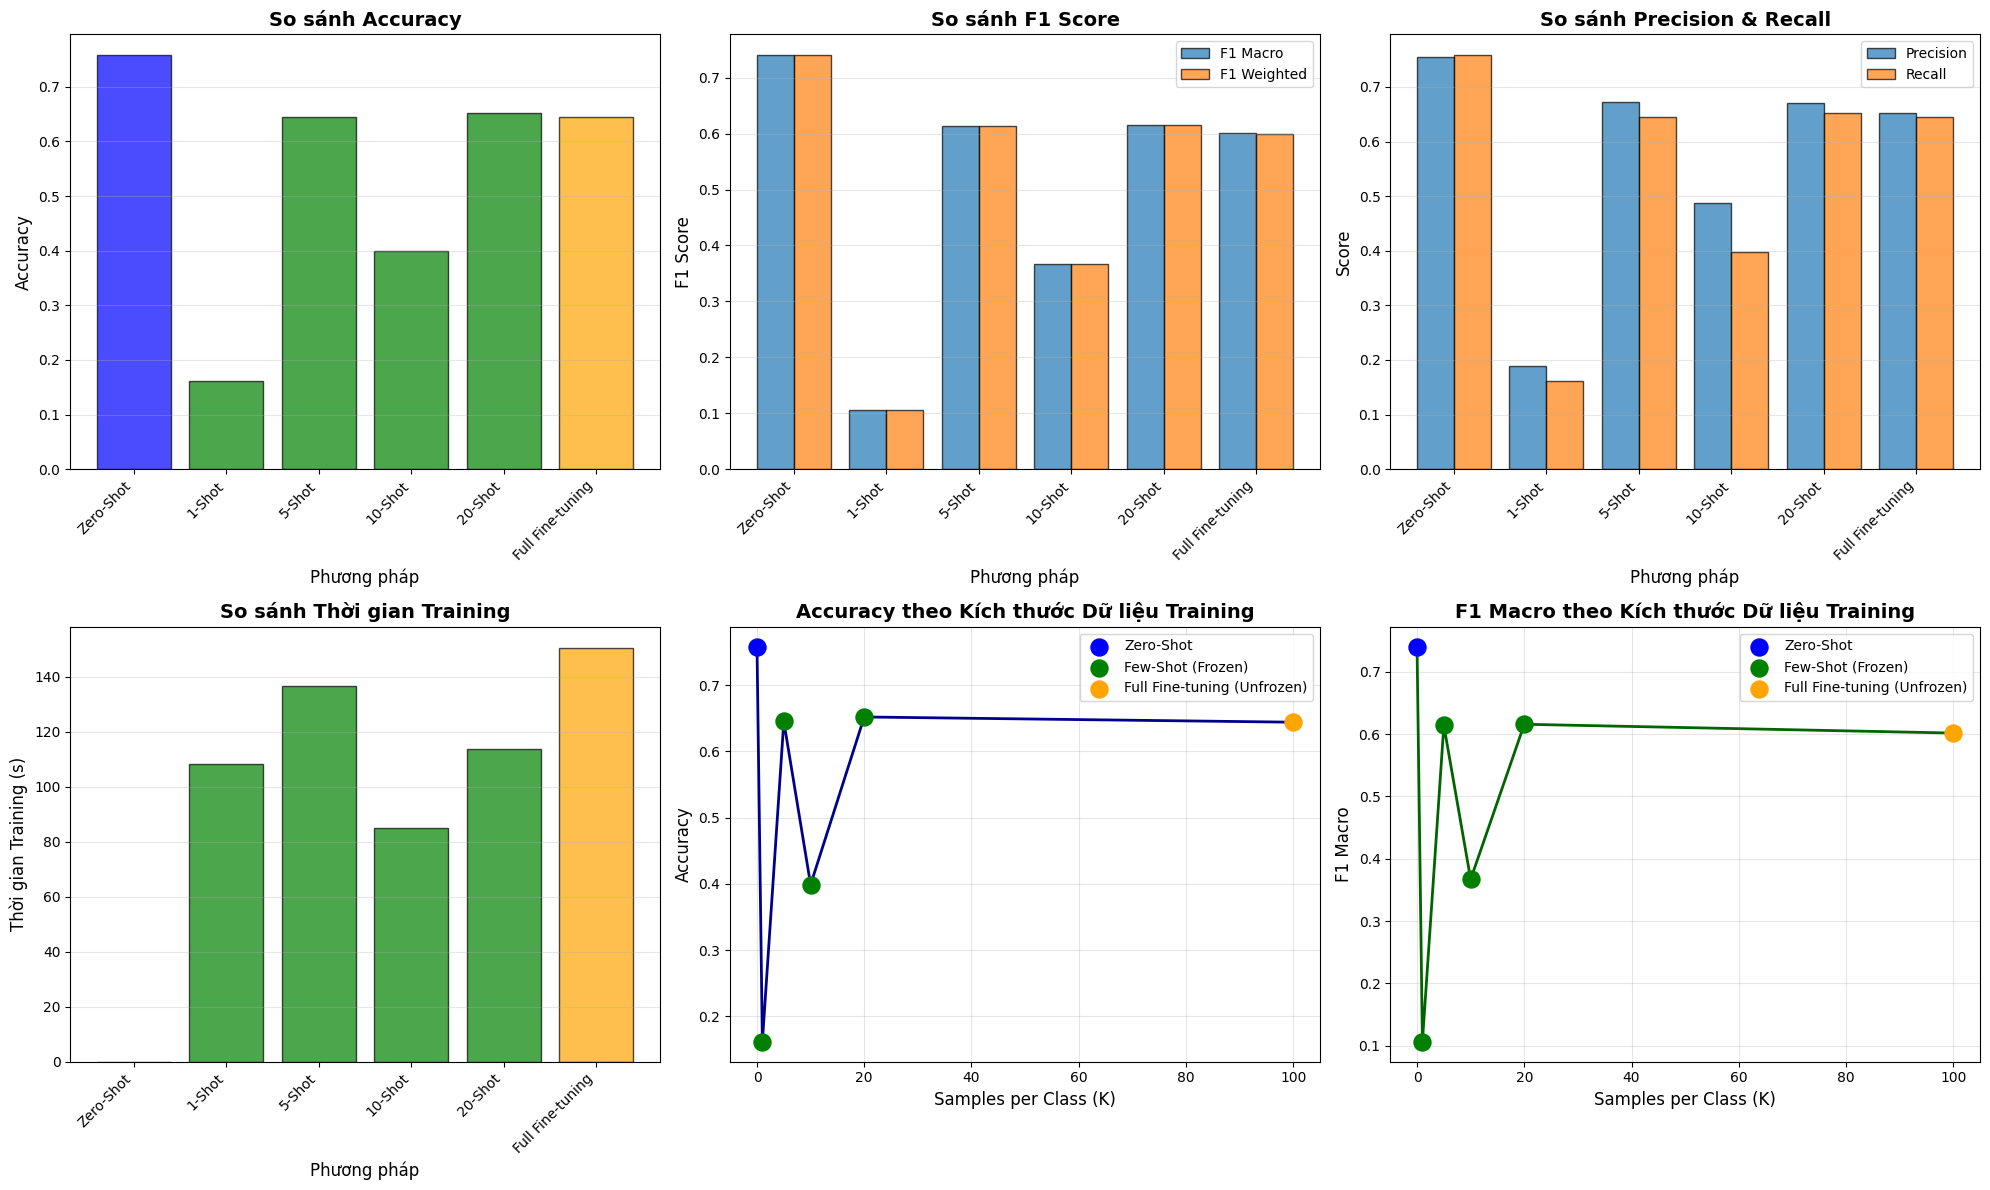
\includegraphics[width=\textwidth]{Images/multimodal_accuracy_vs_k.png}
        \caption{Accuracy theo số lượng samples per class (K)}
        \label{fig:accuracy-vs-k}
    \end{subfigure}
    \hfill
    \begin{subfigure}[b]{0.48\textwidth}
        \centering
        % Placeholder - export from notebook
        % 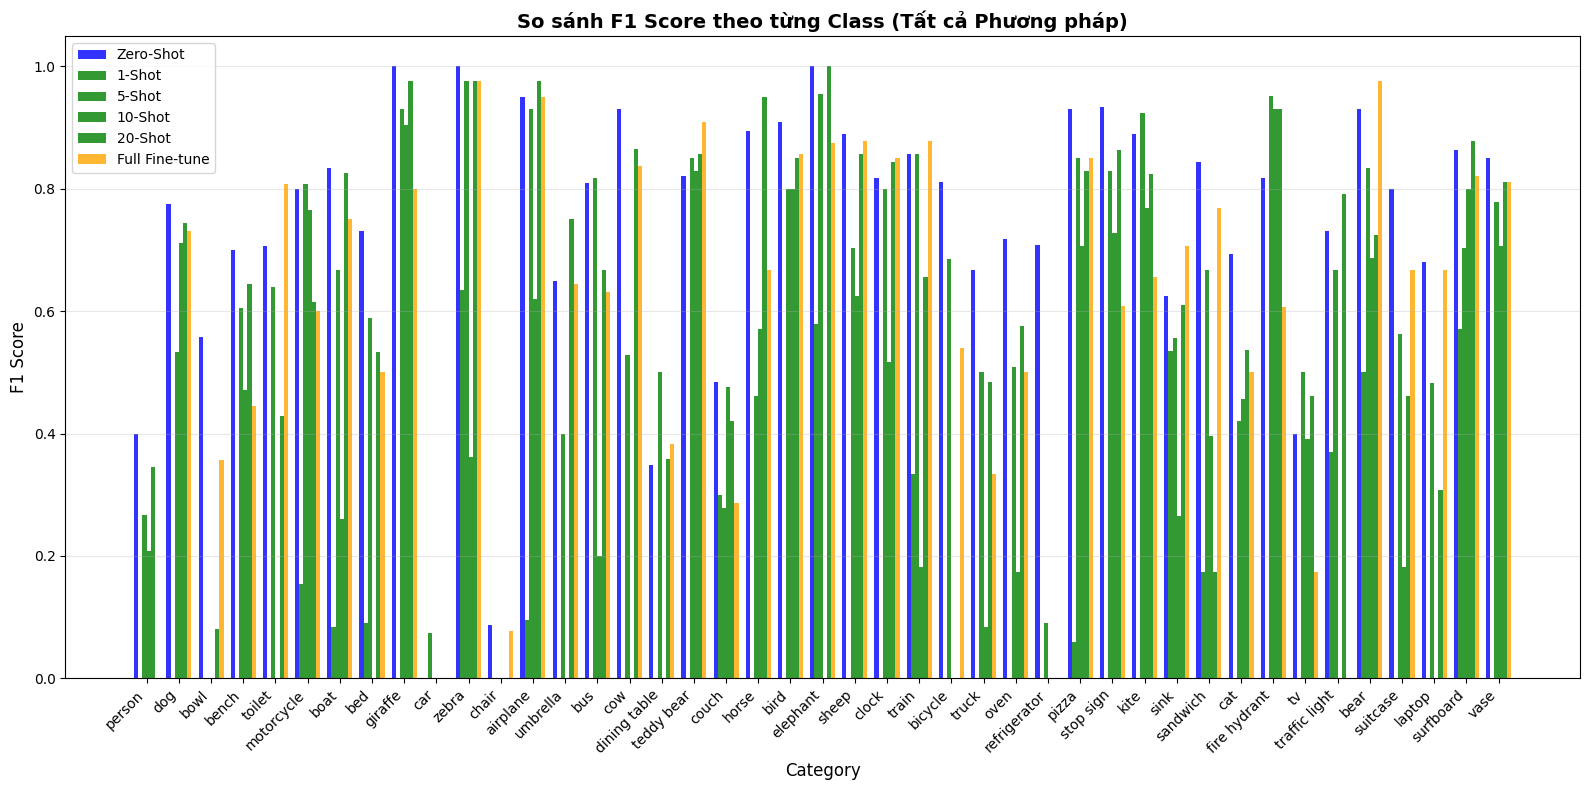
\includegraphics[width=\textwidth]{Images/multimodal_f1_vs_k.png}
        \caption{F1 Macro theo số lượng samples per class (K)}
        \label{fig:f1-vs-k}
    \end{subfigure}
    \caption{Xu hướng thay đổi metrics theo K. Quan sát: performance tăng mạnh từ k=1 đến k=5, sau đó có diminishing returns.}
    \label{fig:metrics-vs-k}
\end{figure}

% After Section: Confusion Matrices
\begin{figure}[H]
    \centering
    \begin{subfigure}[b]{0.32\textwidth}
        \centering
        % Placeholder - export from notebook
        % 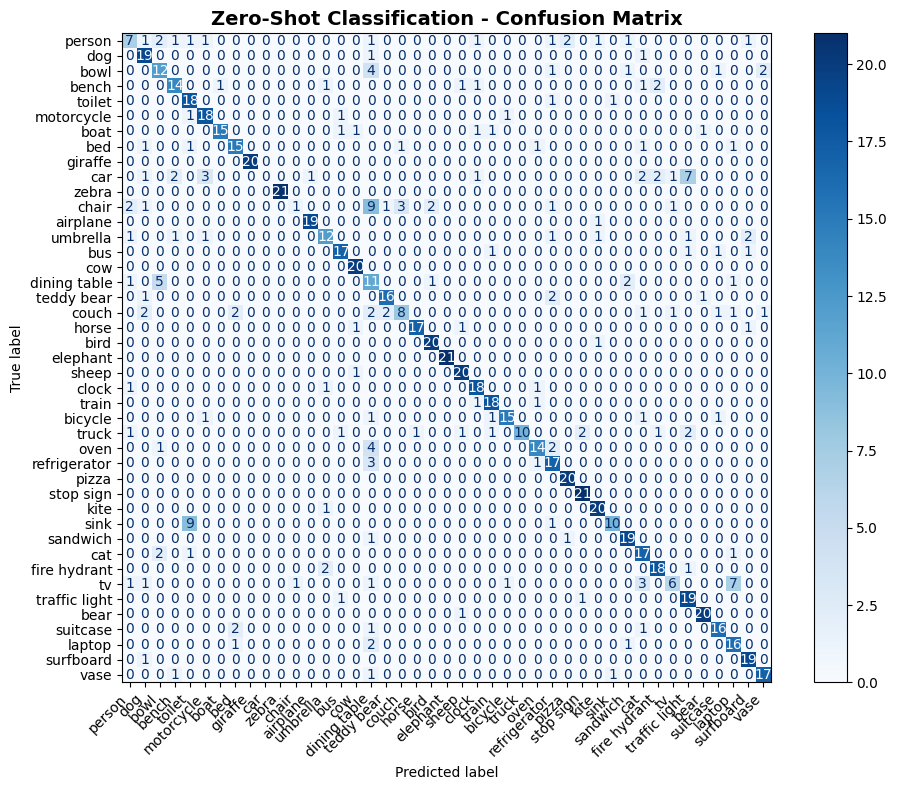
\includegraphics[width=\textwidth]{Images/multimodal_cm_zeroshot.png}
        \caption{Zero-shot (Acc: 75.8\%)}
        \label{fig:cm-zeroshot}
    \end{subfigure}
    \hfill
    \begin{subfigure}[b]{0.32\textwidth}
        \centering
        % Placeholder - export from notebook
        % \includegraphics[width=\textwidth]{Images/multimodal_cm_5shot.png}
        \caption{5-Shot Frozen (Acc: 64.5\%)}
        \label{fig:cm-5shot}
    \end{subfigure}
    \hfill
    \begin{subfigure}[b]{0.32\textwidth}
        \centering
        % Placeholder - export from notebook
        % \includegraphics[width=\textwidth]{Images/multimodal_cm_fullfinetune.png}
        \caption{Full Fine-tune (Acc: 64.4\%)}
        \label{fig:cm-fullfinetune}
    \end{subfigure}
    \caption{Confusion matrices cho ba phương pháp. Zero-shot có đường chéo chính rõ nhất, cho thấy ít confusion giữa các classes.}
    \label{fig:confusion-matrices}
\end{figure}

% After Section: Per-class Performance
\begin{figure}[H]
    \centering
    % Placeholder - export from notebook
    % 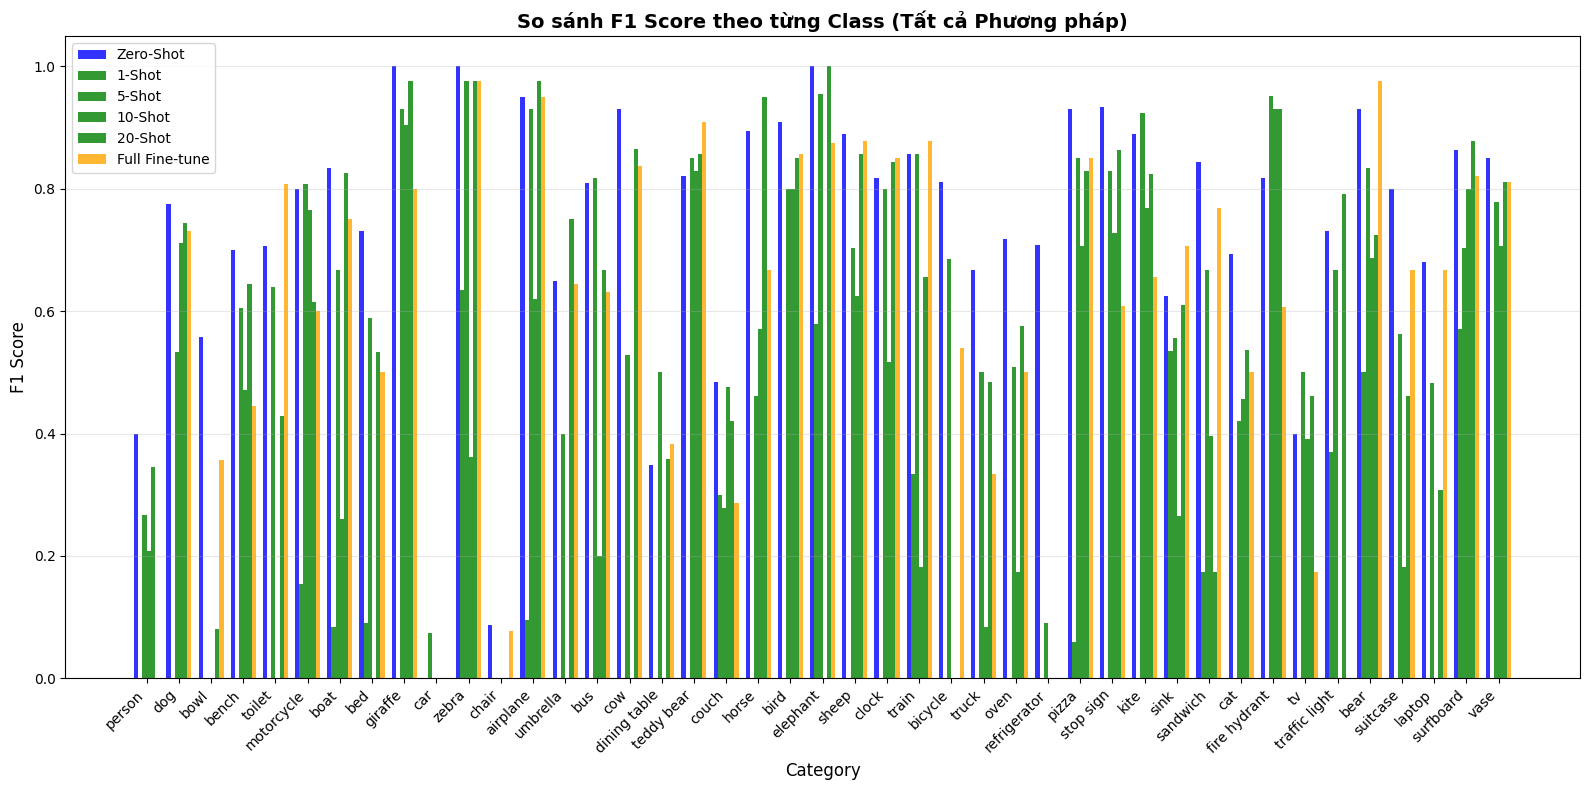
\includegraphics[width=0.95\textwidth]{Images/multimodal_per_class_f1.png}
    \caption{So sánh F1 score theo từng category. Top performers: giraffe, zebra, elephant (distinctive animals). Challenging: chair, person, bowl (varied appearances).}
    \label{fig:per-class-f1}
\end{figure}

% NOTE: To generate these figures from the notebook, add at the end of each plotting cell:
% plt.savefig('report/Images/multimodal_<name>.png', dpi=300, bbox_inches='tight')
%
% Then uncomment the \includegraphics lines above
